\section{Control Function (CF) Estimation of CM Effects}
\label{sec:controlfun}
A conventional approach to estimating CM effects involves a two-stage approach to estimating the ADE and the AIE: the first-stage ($Z_i$ on $D_i$), and the second-stage ($Z_i, D_i$ on $Y_i$).
A CF approach is a simple and intuitive addition to this approach: including the CF terms $\lambda_0, \lambda_1$ in the second-stage regression to address selection-into-mediator.

This section presents two practical estimation strategies.
First, I demonstrate how to estimate CM effects with an assumed distribution of error terms, focusing on the Heckman selection model as the leading case.
Second, I consider a more flexible semi-parametric approach that avoids distributional assumptions --- at the cost of semi-parametrically estimating the corresponding CFs.
While both methods effectively address the selection bias issues detailed in previous sections, they differ in their implementation complexity, efficiency, and underlying assumptions.

\subsection{Parametric CF}
A parametric CF solves the identification problem by assuming a distribution for the unobserved error terms in the first-stage selection model, and modelling selection based on this distribution.
The Heckman selection model is the most pertinent example, assuming the normal distribution for unobserved errors \citep{heckman1979sample}.
A parametric CF using other distributions works in exactly the same manner, replacing the relevant density functions for an alternative distribution as needed.
As such, this section focuses exclusively on the Heckman selection model.\footnote{
    Note that this estimation approach is equivalent to that in the parametric selection model approach to MTEs, in \cite{bjorklund1987estimation}.
}

The Heckman selection model assumes unobserved errors $V_i$ follow a normal distribution, so estimates the first-stage using a probit model.
\[ \Probgiven{D_i = 1}{Z_i, \vec X_i}
    = \Phi \big( \theta + \bar\pi Z_i + \vec\zeta' \vec X_i \big), \]
where $\Phi(.)$ is the cumulative density function for the standard normal distribution, and $\theta, \bar\pi, \vec\zeta$ are parameters estimated with maximum likelihood.
In the parametric case, an excluded instrument ($\vec X_i^{\text{IV}}$) is not technically necessary in the first-stage equation --- though not including one exposes the method to indeterminacy if the errors are not normally distributed.
Thus, it is best practice to use this method with access to an instrument.

From this probit first-stage, construct the inverse Mills ratio terms to serve as the CFs.
These terms capture the correlation between unobserved factors influencing both mediator selection and outcomes, when the errors are normally distributed.
\[ \lambda_0(p') =
        \frac{\phi( - \Phi^{-1}(p') )}{\Phi( -\Phi^{-1}(p') )}, \;\;\;\;
    \lambda_1(p') =
        \frac{\phi( \Phi^{-1}(p') )}{\Phi( \Phi^{-1}(p') )},
        \;\;\;\; \text{ for } p' \in (0,1) \]
where $\phi(.)$ is the probability density function for the standard normal distribution.

Lastly, the second-stage is estimated with OLS, including the CFs with plug in estimates of the mediator propensity score, and $\vec \varphi'$ a linear approximation of nuisance function $\varphi(.)$.
\begin{align*}
    \Egiven{Y_i}{Z_i, D_i, \vec X_i} \;\; =& \;\;
        \alpha
        + \beta D_i
        + \gamma Z_i
        + \delta Z_i D_i
        + \vec \varphi' \vec X_i^- \\
        & \;\; + \rho_0 (1 - D_i) \lambda_0 \big( \hat \pi(Z_i; \vec X_i) \big)
    + \rho_1 D_i \lambda_1\big( \hat \pi(Z_i; \vec X_i) \big)
    + \varepsilon_i,
\end{align*}
where $\hat\pi \big(z';\vec X_i \big)$ are the predictions from the probit first-stage.

The resulting ADE and AIE estimates are composed from sample estimates of the terms in Theorem \ref{thm:cf-identification},
\[ \hat{\text{ADE}}
    = \hat{\gamma} + \hat{\delta}\,\bar D, \;\;\;\;
    \hat{\text{AIE}}
    = \hat{\bar\pi}\; \Big(
        \hat{\beta} + \hat{\delta}\,\bar Z
        + \big(\hat \rho_1 - \hat \rho_0 \big)
        \frac1N \sum_{i=1}^N \Gamma \big( \hat\pi(0;\vec X_i), \hat\pi(1;\vec X_i)\big) \Big) \]
where $\bar D = \frac1N \sum_{i=1}^N D_i$, $\bar Z = \frac1N \sum_{i=1}^N Z_i$,
$\hat{\bar\pi}$ is the estimate of the mean compliance rate, and $\frac1N \sum_{i=1}^N \Gamma(.,.)$ is the average of the complier adjustment term as a function of $\lambda_1$ with $\hat\pi \big(0; \vec X_i \big), \hat\pi \big(1; \vec X_i \big)$ values plugged in.

The standard errors for estimates can be computed using the delta method.
Specifically, accounting for both the sampling variability in the first-stage estimates of the mediator propensity score as well as the second-stage sampling variability.
This approach yields $\sqrt{n}$-consistent estimates when the underlying error terms follow a bivariate normal distribution --- i.e., when $\pi(Z_i; \vec X_i)$ is correctly modelled by the probit first-stage.
Errors can also be estimated by the bootstrap, by including estimation of both the first and second-stage within each bootstrap iteration.
% \aref{appendix:implement} further describes the implementation of this approach in the R language \citep{R2023}, with a linear probit first-stage and second-stage estimated by OLS.

In practice, a parametric CF approach is simple to implement using standard statistical packages.
The key advantage is computational simplicity and efficiency, particularly in moderate-sized samples.
However, this comes at the cost of strong distributional assumptions.
For example, if the error terms deviate substantially from joint normality, the estimates may be biased.\footnote{
    While this concern is immaterial in an IV setting estimating the LATE \citep{kline2019heckits}, it is pertinent in this setting as the CF extrapolates from IV compliers to mediator compliers.
}

\subsection{Semi-parametric CF}
For settings where researchers are not comfortable specifying a specific distribution for the error terms, a semi-parametric CF will nonetheless consistently estimate CM effects.
This method maintains the same identification strategy but avoids assuming a specific error distribution.

The semi-parametric approach begins with flexible estimation of the first-stage, estimating the mediator propensity score,
\[ \Probgiven{D_i = 1}{Z_i, \vec X_i}
    = \pi\left(Z_i; \vec X_i \right), \]
where $\vec X_i$ must include the instrument(s) $\vec X_i^{\text{IV}}$.
This can be estimated using flexible methods, as long as the first-stage is estimated $\sqrt{n}$-consistently.\footnote{
    If an estimate of the first-stage that is not $\sqrt{n}$-consistent is used (e.g., a modern machine learning estimator), then the resulting second-stage estimate will not be $\sqrt{n}$-consistent.
    %This could be ameliorated by augmenting the approach with cross-fitting, and the appropriate Neyman orthogonal moments; \cite{bia2024double} use this approach for one-sided selection problems, but (as fas as I am aware) there is no general double machine learning approach for CF methods with a two-sided selection problem.
}
An attractive option is the \cite{klein1993efficient} semi-parametric binary response model, which avoids relying on an assumed distribution of first-stage errors though requires a linear specification.
If it is important to avoid a linear specification, then a probability forest avoids linearity assumptions \citep{athey2019generalized} --- though is best used for cases with many columns in the $\vec X_i$ variables.

The second-stage is estimated with semi-parametric methods.
Consider the subsamples of mediator refusers and takers separately,
\begin{align*}
    \Egiven{Y_i}{Z_i, D_i = 0, \vec X_i} &=
        \alpha + \gamma Z_i + \varphi\big( \vec X_i^- \big)
        + \rho_0 \lambda_0 \big( \pi(Z_i ; \vec X_i) \big), \\
    \Egiven{Y_i}{Z_i, D_i = 1, \vec X_i} &=
        (\alpha + \beta) + (\gamma + \delta) Z_i + \varphi\big( \vec X_i^- \big)
        + \rho_1 \lambda_1 \big( \pi(Z_i ; \vec X_i) \big).
\end{align*}
The separated subsamples can be estimated, each individually, with semi-parametric methods.
The linear parameters (including a linear approximation $\vec \varphi'$ of nuisance function $\varphi(.)$)\footnote{
    Appropriate interactions between $Z_i, D_i$ and $\vec X_i$ can also flexibly control for $\vec X_i$, again avoiding linearity assumptions.
} can be estimated with OLS, while $\rho_0 \lambda_0$ and $\rho_1 \lambda_1$ take a flexible semi-parametric specification with first-stage estimates $\hat \pi(Z_i; \vec X_i)$ plugged in.
An attractive option is a series estimator, such as a spline specification, as this estimates the function without assuming a functional form but maintains $\sqrt n$-consistency.

The ADE is estimated by this approach as follows.
Take $\hat \gamma$, the $D_i = 0$ subsample estimate of $\gamma$, and $(\hat{\gamma + \delta})$, the $D_i = 1$ subsample estimate of $(\gamma + \delta)$, to give
\[ \hat{\text{ADE}}^{\text{CF}}
    = (1 - \bar D) \, \hat \gamma + \bar D \, (\hat{\gamma + \delta}). \]

The AIE is less simple, for two reasons that differ from the parametric CF setting.
First, the intercepts for each subsample, $\alpha$ and $(\alpha + \beta)$, are not separately identified from the CFs if the $\lambda_0, \lambda_1$ functions are flexibly estimated.
Second, a semi-parametric specification for the CFs mean $\rho_0$ and $\lambda_0$ are no longer separately identified from each other (and same for $\rho_1,\lambda_1$).
As such, it is not possible to directly use $\hat \lambda_0, \hat \lambda_1$ in estimating the complier adjustment term (as is done in the parametric case).

Theses problem can be avoided by estimating the AIE using its relation to the ATE.
Write $\hat{\text{ATE}}$ for the point-estimate of the ATE, and 
$\hat\delta = (\hat{\gamma + \delta}) - \hat\gamma$ for the point estimate of $\delta$, to give the following estimator,
\[ \hat{\text{AIE}}^{\text{CF}}
    = \hat{\text{ATE}}
    - (1 - \bar Z) \, \left( 
        \frac 1N \sum_{i = 1}^N \hat\gamma + \hat \delta \, \hat\pi(1; \vec X_i) \right)
    - \bar Z \, \left(
        \frac 1N \sum_{i = 1}^N \hat\gamma + \hat \delta \, \hat\pi(0; \vec X_i)  \right), \]
where $\frac 1N \sum_{i = 1}^N \hat\gamma + \hat \delta \, \hat\pi(0; \vec X_i)$ estimates the ADE conditional on $Z_i = 0$, $\E{\gamma + \delta D_i(0)}$, and $\frac 1N \sum_{i = 1}^N \hat\gamma + \hat \delta \, \hat\pi(1; \vec X_i)$ estimates the ADE conditional on $Z_i = 1$, $\E{\gamma + \delta D_i(1)}$.
\aref{appendix:semi-parametric} describes the reasoning for this estimator of the AIE, relative to estimates of the ATE and ADE, in further detail.
% \aref{appendix:implement} describes in further detail the implementation of this approach in the R language \citep{R2023}, with a \cite{klein1993efficient} first-stage and splines in the second-stage CF estimation.

The ideal instrument $\vec X_i^{\text{IV}}$ for this semi-parametric approach is continuous, and varies $\pi(z'; \vec X_i)$ between 0 and 1 for every value of $z', \vec X_i^-$ (identification at infinity).
In practice, it is unlikely to find IV(s) that satisfy this condition.
In this case, the \cite{brinch2017beyond} restricted approach can be used for estimation --- even with a categorical instrument and no control variables.
This amounts to limiting the number of parameters in the semi-parametric CF estimation to the number of discrete values that $\pi(z'; \vec X_i)$ takes minus one, changing little to the estimation strategy.

This semi-parametric approach achieves valid estimation of the CM effects, without specifying the distribution behind unobserved error terms, and achieves desirable properties as long as the first-stage correctly estimates the mediator propensity score, and the structural assumptions hold true.
The standard errors for estimates can again be computed using the delta method, or estimated by the bootstrap --- again, across both first and second-stages within each bootstrap iteration.
Note that relying on propensity score estimation requires assumptions that can be found wanting in real-world settings; a common support condition for the mediator is required, and a semi-/non-parametric first-stage may become cumbersome if there are many control variables or many rows of data.

\subsection{Simulation Evidence}
\label{sec:simulations}
The following simulation gives an example to show how these methods work in practice.
Suppose data observed to the researcher $Z_i, D_i, Y_i, \vec X_i$ are drawn from the following data generating processes, for $i = 1, \hdots, N$, with 
$N = 1,000$ for this simulation.
\[ Z_i \sim \text{Binom}\left(0.5 \right),
    \;\; \vec X_i^- \sim N(4, 1),
    \;\; \vec X_i^{\text{IV}} \sim \text{Uniform}\left( -1, 1 \right),
    \;\; \left( U_{0,i}, U_{1,i}, U_{C,i} \right) \sim
    N\left( \vec 0, \mat \Sigma \right) \]
$\mat \Sigma$ is the matrix of parameters which controls the level of confounding from unobserved costs and benefits.\footnote{
    The correlation and relative standard deviations for $U_{0,i}, U_{1,i}$ affect how large selection bias in conventional CM estimates; correlation for these with unobserved costs $U_{C,i}$ does not particularly matter, though increased variance in unobserved costs makes estimates less precise for both OLS and CF methods.
}

Each $i$ chooses to take mediator $D_i$ by a Roy model, with following mean definitions for each $z', d' = 0, 1$
\begin{align*}
    D_i(z') &= \indicator{C_i \leq Y_i(z', 1) - Y_i(z', 0)},  \\
    \mu_{d'}\left(z' ; \vec X_i \right) &= \left( z' + d' + z' d' \right) + \vec X_i^-,
    \;\; \mu_{C}\left(z' ; \vec X_i \right) = 3z' + \vec X_i^- - \vec X_i^{\text{IV}}.
\end{align*}
Following \autoref{sec:regression}, these data have the following first and second-stage equations:
\begin{align*}
    D_i &= \indicator{U_{C,i} - \big( U_{1,i} - U_{0,i} \big)
    \leq -3Z_i + \vec X_i^- - \vec X_i^{\text{IV}}},  \\
    Y_i &= Z_i + D_i + Z_i D_i + \vec X_i^-
        + \left( 1 - D_i \right) U_{0,i} + D_i U_{1,i}.
\end{align*}
Treatment $Z_i$ has a causal effect on outcome $Y_i$, and it operates partially through mediator $D_i$.
Outcome mean $\mu_{D_i}\left( Z_i; \vec X_i \right)$ contains an interaction term, $Z_i D_i$, so while $Z_i,D_i$ have constant partial effects, the ATE depends on how many $i$ choose to take the mediator so there is treatment effect heterogeneity.

After $Z_i$ is assigned, $i$ chooses to take mediator $D_i$ by considering the costs and benefits --- which vary based on $Z_i$, demographic controls $\vec X_i$, and the (non-degenerate) unobserved error terms $U_{i,0}, U_{1,i}$.
As a result, sequential ignorability does not hold; the mediator is not conditionally ignorable.
Thus, a conventional approach to CM does not give an estimate for how much of the ATE goes through mediator $D$, but is contaminated by selection bias thanks to the unobserved error terms.

I simulate this data generating process 10,000 times, using $\mat\Sigma =
\left(\begin{smallmatrix} 1 & 0.75 & 0 \\ 0.75 & 2.25 & 0 \\ 0 & 0 & 0.25 \end{smallmatrix}\right)$,\footnote{
    This choice of parameters has $\Var{U_{0,i}} = 1, \Var{U_{1,i}} = 2.25, \text{Corr}\big(U_{0,i}, U_{1,i}\big) = 0.5$ so that unobserved errors meaningfully confound conventional CM methods, with notable heteroscedasticity.
    Unobserved costs are uncorrelated with $U_{0,i}, U_{1,i}$ (although non-zero correlation would not meaningfully change the results), and $\Var{U_{C,i}} = 0.25$ maintains uncertainty in unobserved costs.
}
and estimate CM effects with conventional CM methods (two-stage OLS) and the introduced CF methods.
In this simulation $\Prob{D_i = 1} = 0.379$, and $65.77\%$ of the sample are mediator compliers (for whom $D_i(0)=0$ and $D_i(1)=1$).
This gives an ATE value of 2.60, ADE 1.38, and AIE 1.22, respectively.\footnote{
    Note that ATE $=$ ADE $+$ AIE in this setting.
    $\Prob{Z_i=1} = 0.5$ ensures this equality, but it is not guaranteed in general.
    See \aref{appendix:semi-parametric}.
}

\begin{figure}[h!]
    \caption{Simulated Distribution of CM Effect Estimates, Semi-parametric versus OLS, Relative to True Value.}
    \begin{subfigure}[c]{0.475\textwidth}
        \centering
        \caption{$\hat{\text{ADE}} - \text{ADE}$.}
        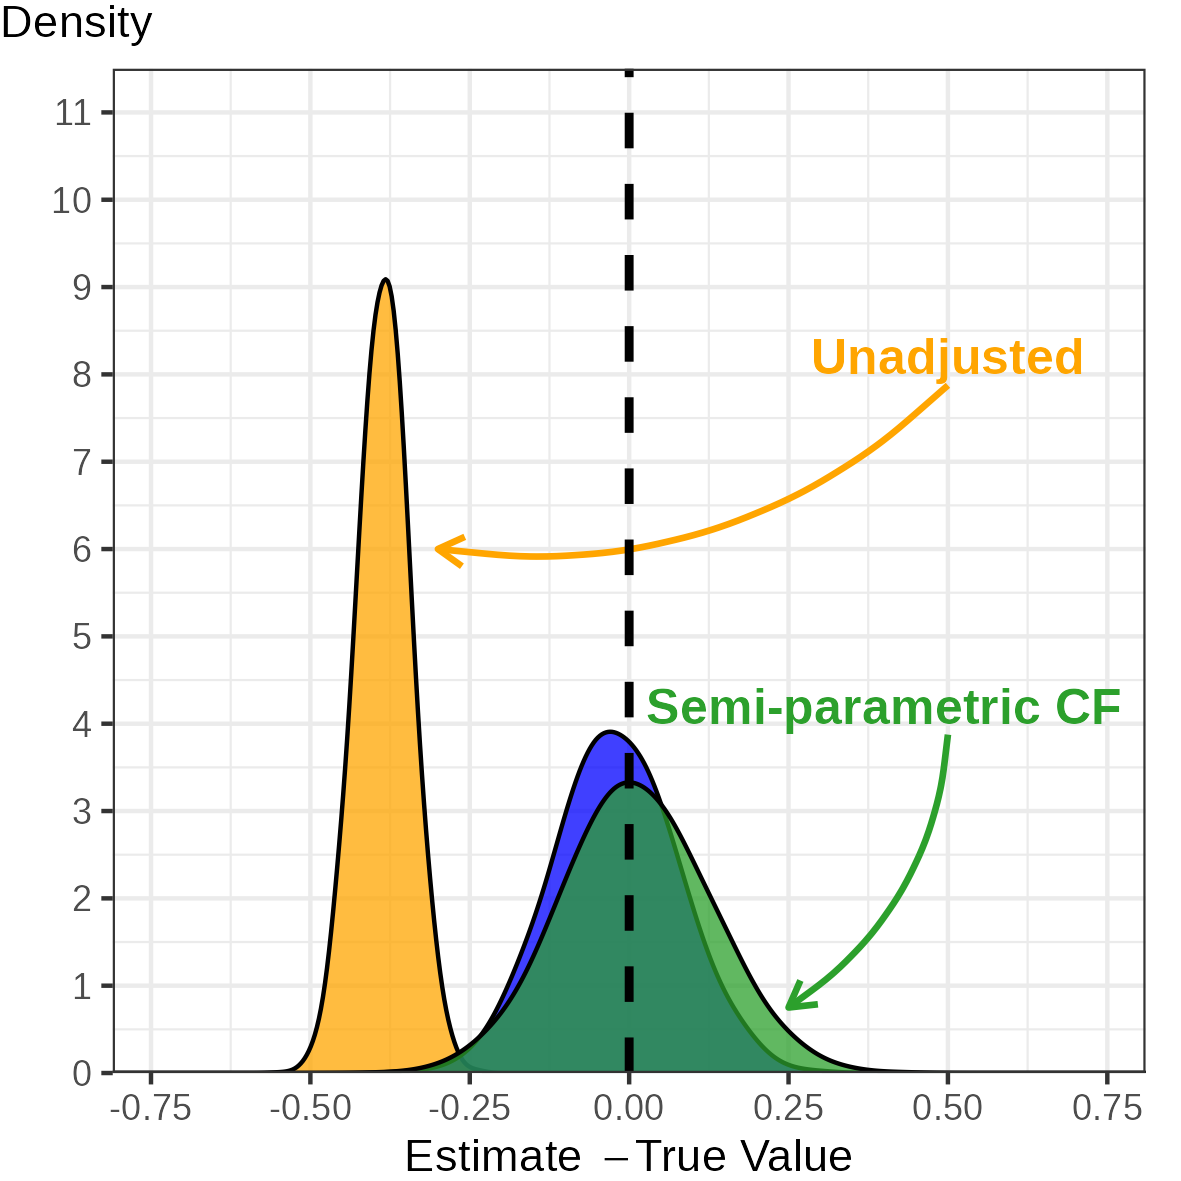
\includegraphics[width=\textwidth]{
            ../programs/simulations/sim-output/uniform-direct-dist.png}
    \end{subfigure}
    \begin{subfigure}[c]{0.475\textwidth}
        \centering
        \caption{$\hat{\text{AIE}} - \text{AIE}$.}
        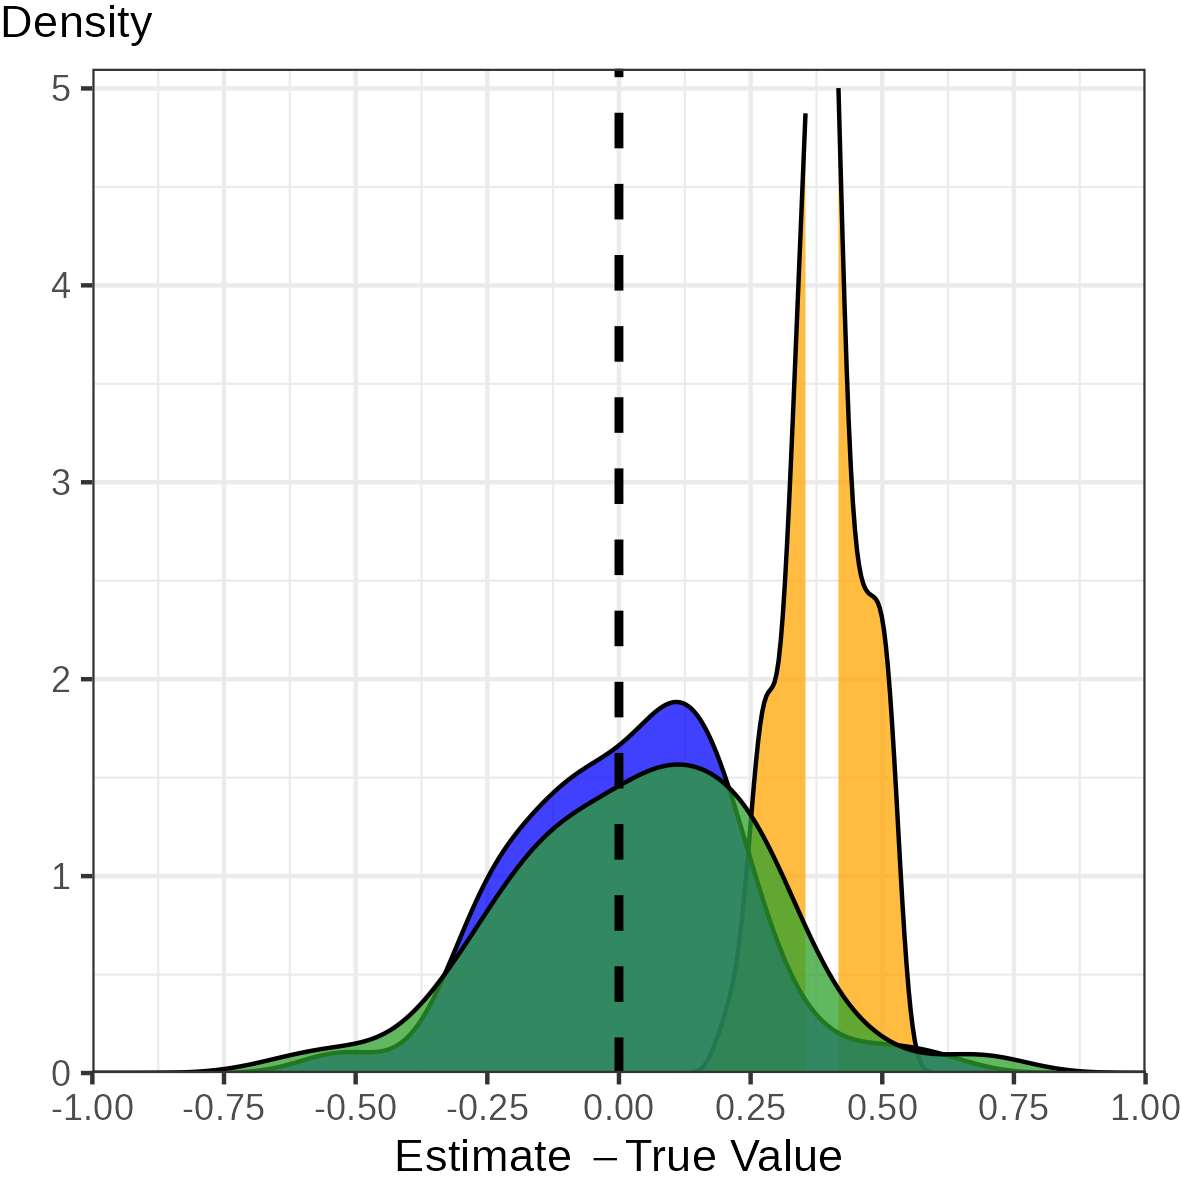
\includegraphics[width=\textwidth]{
            ../programs/simulations/sim-output/uniform-indirect-dist.png}
    \end{subfigure}
    \label{fig:cm-uniform-dist}
    \justify
    \footnotesize    
    \textbf{Note:}
    These figures show the empirical density of point estimates minus the true average effect, for 10,000 different datasets generated from a Roy model with correlated uniformly distributed error terms.
    The black dashed line is the true value;
    orange is the distribution of conventional CM estimates from two-stage OLS \citep{imai2010identification},
    and green estimates with a two-stage semi-parametric CF.
\end{figure}

\autoref{fig:cm-normal-dist} shows how these estimates perform, with a parametric CF approach, relative to the true value.
The OLS estimates' distribution do not overlap the true values for any standard level of significance; the distance between the OLS estimates and the true values are the underlying bias terms derived in \autoref{thm:selection-bias}.
The parametric CF approach perfectly reproduces the true values, as the probit first-stage correctly models the normally distributed error terms.
The semi-parametric approach (not shown in \autoref{fig:cm-normal-dist}) performs similarly, with a wider distribution; this is to be expected comparing a correctly specified parametric model with a semi-parametric one.

The parametric CF may not be appropriate in setting with non-normal error terms.
I simulated the same data again, but transform $U_{0,i}, U_{1,i}$ to be correlated uniform errors (with the same standard deviations as previously).
\autoref{fig:cm-uniform-dist} shows the resulting distribution of point-estimates, relative to the truth, for the parametric and semi-parametric approaches.
The parametric CF is slightly off target, showing persistent bias from incorrectly specifying the error term distribution.
The semi-parametric approach is centred exactly around the truth, with a slightly high variance (as is expected).

\begin{figure}[h!]
    \caption{CF Adjusted Estimates Work with Different Error Term Parameters.}
    \begin{subfigure}[c]{0.475\textwidth}
        \centering
        \caption{ADE.}
        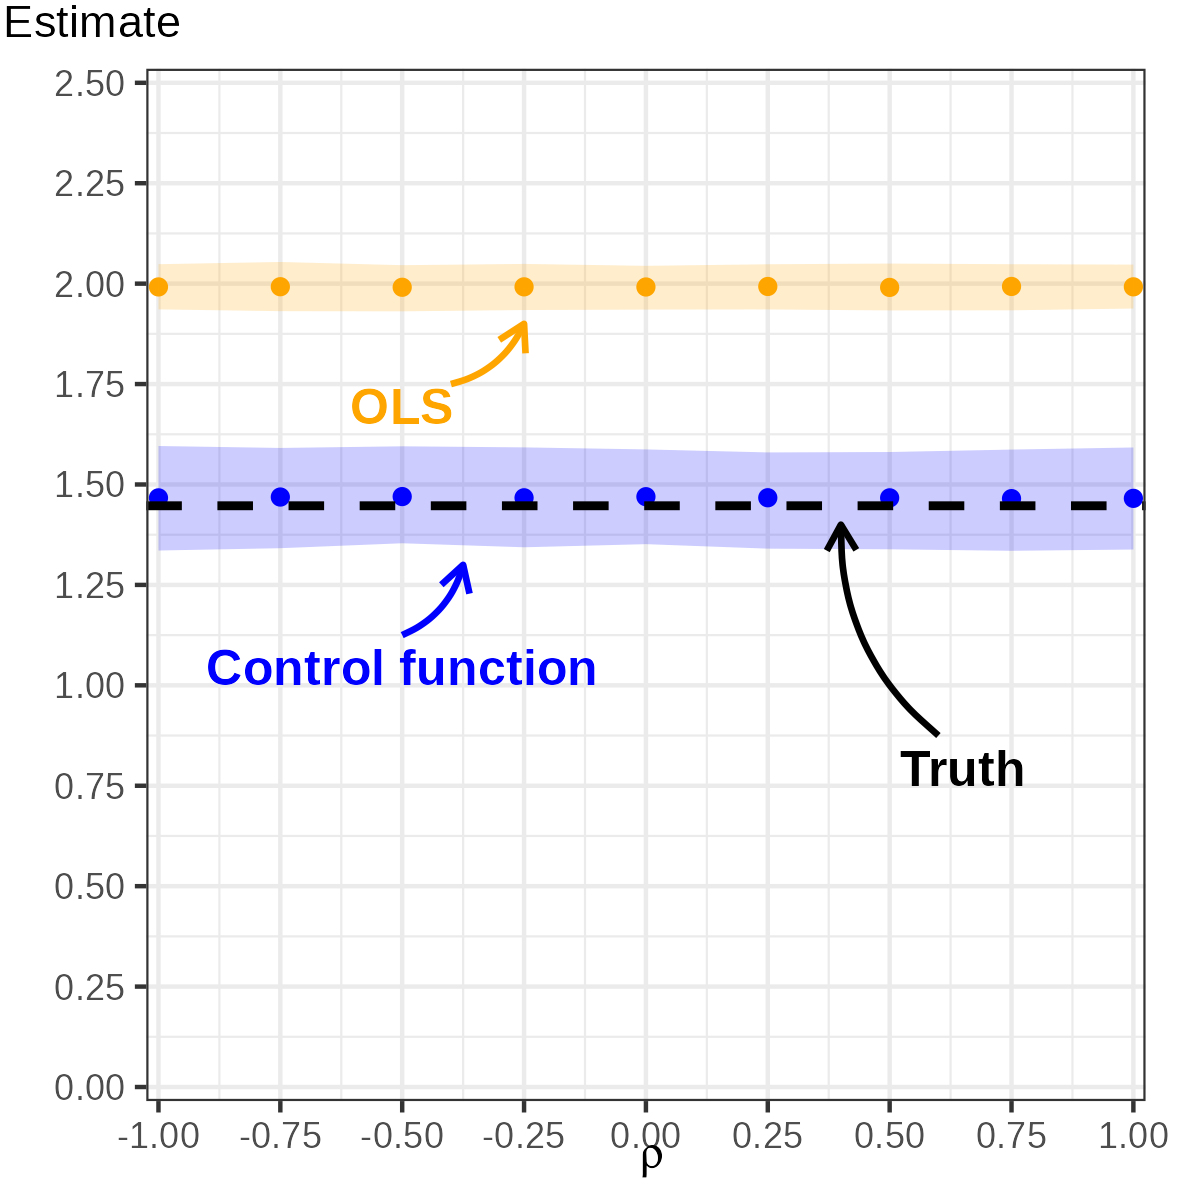
\includegraphics[width=\textwidth]{
            ../programs/simulations/sim-output/rho-directeffect-bias.png}
    \end{subfigure}
    \begin{subfigure}[c]{0.475\textwidth}
        \centering
        \caption{AIE.}
        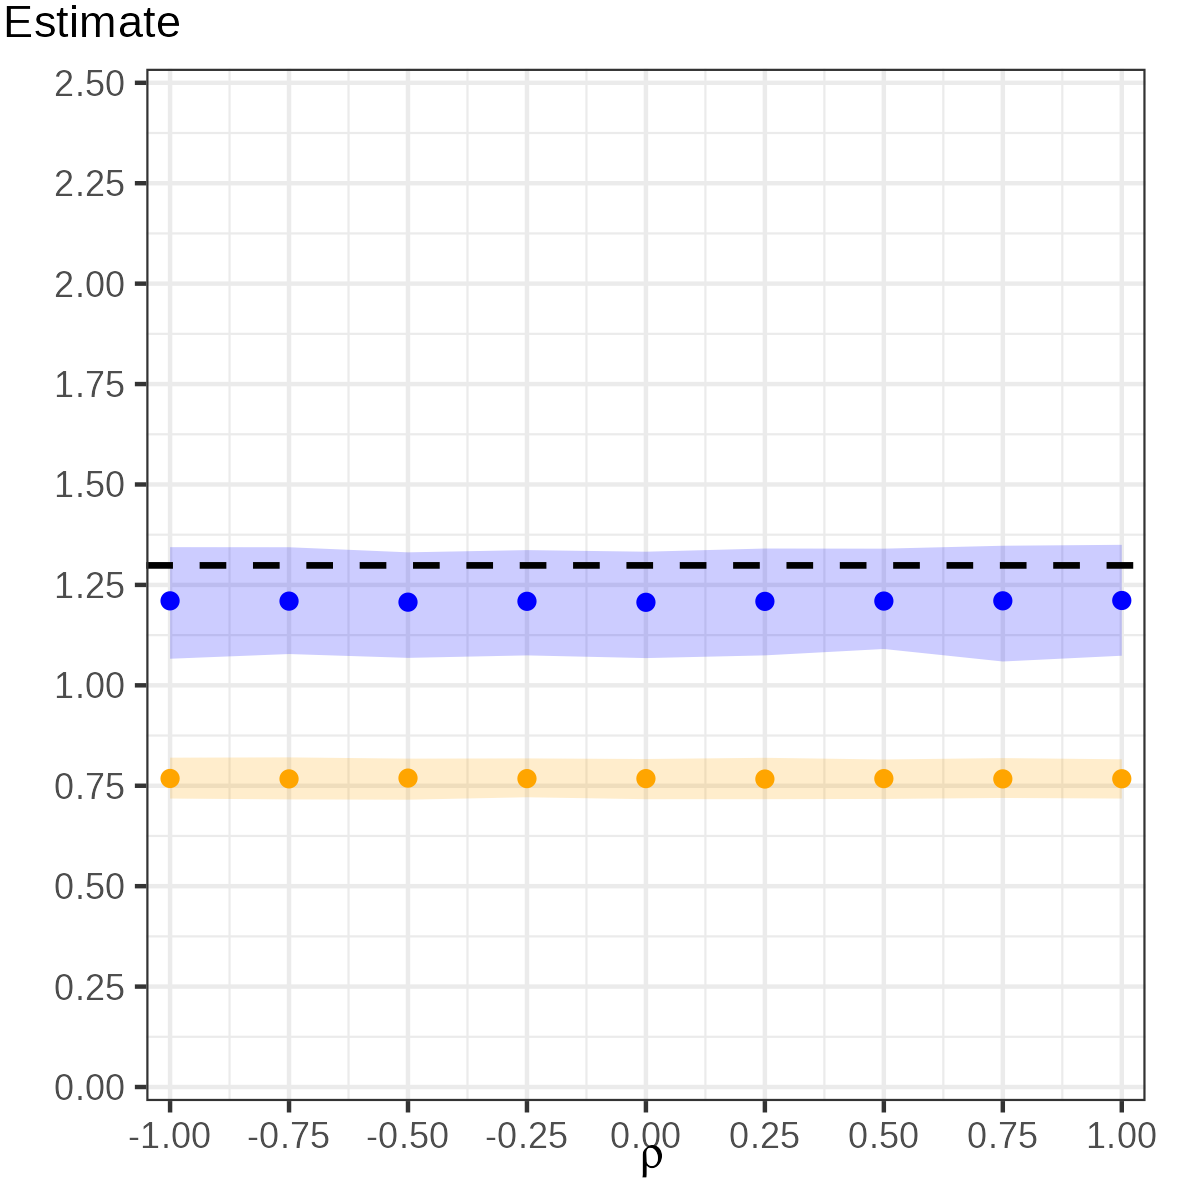
\includegraphics[width=\textwidth]{
            ../programs/simulations/sim-output/rho-indirecteffect-bias.png}
    \end{subfigure}
    \label{fig:rho-bias}
    \justify
    \footnotesize    
    \textbf{Note:}
    These figures show the OLS and CF point estimates of the ADE and AIE, for $N = 1,000$ sample size, varying $\text{Corr}\big(U_{0,i}, U_{1,i}\big)$ values with $\Var{U_{0,i}} = 1, \Var{U_{1,i}} = 1.5$ fixed.
    The black dashed line is the true value, coloured points are points estimates for the respective data generated, and shaded regions are the 95\% confidence intervals from 1,000 bootstraps each.
    Orange represents OLS estimates, blue the CF approach.
\end{figure}

The error terms determine the bias in OLS estimates of the ADE and AIE, so the bias varies for different values of the error-term parameters $\text{Corr}\big(U_{0,i}, U_{1,i}\big) \in [-1, 1]$ and $\Var{U_{0,i}}, \Var{U_{1,i}} \geq 0$.
The true AIE values vary, because $D_i(Z_i)$ compliers have higher average values of $U_{1,i} - U_{0,i}$ as $\text{Corr}\big(U_{0,i}, U_{1,i}\big)$ increases.
\autoref{fig:rho-bias} shows CF estimates against estimates calculated by standard OLS, showing 95\% confidence intervals calculated from 1,000 bootstraps.
The point estimates of the CF do not exactly equal the true values, as they are estimates from one simulation (not averages across many generated datasets, as in \autoref{fig:cm-uniform-dist}).
The CF approach improves on OLS estimates by correcting for bias, with confidence regions overlapping the true values.\footnote{
    In the appendix, \autoref{fig:sigma-1-bias} shows the same simulation while varying $\Var{U_{1,i}}$, with fixed $\Var{U_{0,i}} = 1, \text{Corr}\big(U_{0,i}, U_{1,i}\big) = 0.5$.
    The conclusion is the same as for varying the correlation coefficient, $\rho$, in \autoref{fig:rho-bias}.
}
This correction did not come for free: the standard errors are significantly greater in a CF approach than OLS.
In this manner, this simulation shows the pros and cons of using the CF approach to estimating CM effects in practice.
